\documentclass{article}


\usepackage[utf8]{inputenc}
% \usepackage[utf8]{inputenc}
\usepackage{multicol}
\usepackage{dcolumn}
\usepackage[a4paper,top=3cm,bottom=3cm,left=2cm,right=2cm,marginparwidth=1.75cm]{geometry}
\usepackage{multicol}
\usepackage{multirow}
\usepackage{amsmath}
\usepackage{graphicx}
\usepackage{hyperref}
\hypersetup{colorlinks=true,linkcolor=black,filecolor=magenta,urlcolor=cyan,}
\usepackage{amsfonts}
\usepackage{mathtools}
\usepackage{lipsum}
\usepackage{float}
\usepackage{layout}
\usepackage{bm}

\begin{document}



%TitlePage%TitlePage%TitlePage%TitlePage%TitlePage%TitlePage%TitlePage%TitlePage%TitlePage%TitlePage%TitlePage%TitlePage%TitlePage
\newgeometry{top=4cm,bottom=2.5cm,left=4cm,right=4cm}
\begin{titlepage}

    \begin{center}
    
    
    
    \textup{\Large {\bf Summer Internship Project} \\ Report}\\[0.3in]
    
    % Title
    \Large \textbf {Detection of Cosmic Muons Using Gas Detectors}\\[0.7in]
    
    
           
    
    % Submitted by
    \normalsize Submitted by \\[0.2in]
    \textbf{Anantha Padmanabhan M Nair}\\
    \normalsize
    $4^{th}$ year Int. MSc Student\\[0.1in]
    
    
\includegraphics[width=0.25 \textwidth]{NISER.png}\\[0.1in]
    \Large{School of Physical Sciences}\\
    \normalsize
    \textsc{National Institute of Science Education and Research},\\
    Tehsildar Office, Khurda\\
    Pipli, Near, Jatni, Odisha 752050\\
    
    
    
    
    
    \vspace{.2in}
    Under the guidance of\\[0.2in]
    \textbf{Dr. Sanjib Muhuri}\\
    Scientific Officer
    
    
    
    \vspace{.3in}
    
    % Bottom of the page
    
\includegraphics[width=0.2\textwidth]{VECC.png}\\[0.1in]
    \Large{Experimental High Energy Physics}\\
    \normalsize
    \textsc{Variable Energy Cyclotron Centre}\\
    1/AF, \\Bidhannagar, Kolkata, \\West Bengal, 700064 \\
    \vspace{0.2in}
    Summer Internship 2023
    
    \end{center}
    
\end{titlepage}
\restoregeometry
%TitlePage%TitlePage%TitlePage%TitlePage%TitlePage%TitlePage%TitlePage%TitlePage%TitlePage%TitlePage%TitlePage%TitlePage%TitlePage%









%Acknowledgements%Acknowledgements%Acknowledgements%Acknowledgements%Acknowledgements%Acknowledgements%Acknowledgements%Acknowledgements
\newgeometry{top=4.5cm,bottom=3.5cm,left=3cm,right=3cm}
\cleardoublepage
\begin{center}
    \Large{\textbf{Acknowledgements}}
\end{center}

\vspace{0.2in}
I would like to express my sincere gratitude to Dr. Sanjib Muhuri, 
my guide and mentor, for his invaluable support, guidance, 
and expertise throughout my internship on the simulation and 
experimental detection of cosmic muons using the ALICE detector. 
His vast knowledge and constant encouragement have been instrumental 
in shaping my understanding of this complex field of study.
I am also grateful to the High Energy Group at VECC (Variable 
Energy Cyclotron Centre) for providing me with the necessary 
resources, infrastructure, and access to the ALICE detector. Their 
assistance and cooperation have been vital in carrying out the 
experimental phase of this internship.
I extend my heartfelt appreciation to the Department of School of 
Physical Sciences at NISER (National Institute of Science Education 
and Research) for providing me with the opportunity to pursue this 
internship. The conducive academic environment and the support of the 
faculty have greatly contributed to my overall learning experience.
I would like to acknowledge the collective efforts of the researchers, 
technicians, and staff members who have been associated with the 
project. Their contributions, suggestions, and collaboration have 
significantly enriched my internship journey.
Lastly, I express my gratitude to my fellow interns and 
friends for their camaraderie, stimulating discussions, and 
continuous encouragement. Their presence has made this internship 
an enjoyable and enriching experience.
In conclusion, I am immensely thankful to all individuals 
and institutions mentioned above for their unwavering support, 
guidance, and contributions, which have been instrumental in the 
successful completion of this internship.
\newpage
\restoregeometry
%Acknowledgements%Acknowledgements%Acknowledgements%Acknowledgements%Acknowledgements%Acknowledgements%Acknowledgements%Acknowledgements











%Certificate%Certificate%Certificate%Certificate%Certificate%Certificate%Certificate%Certificate%Certificate%Certificate%Certificate%Certificate
\newgeometry{top=4.5cm,bottom=3.5cm,left=4cm,right=4cm}
\newpage
\thispagestyle{empty}

\begin{center}

\huge{\textsc{Variable Energy Cyclotron Centre, Kolkata}}\\[1cm]
\normalsize

\emph{\LARGE Certificate}\\[1cm]
\end{center}



This is to certify that Mr. Anantha Padmanabhan M Nair, a 
student of the National Institute of Science Education and 
Research (NISER), has successfully completed a summer internship 
in the field of Cosmic Muons and its Detection by ALICE Detectors. 
The internship was conducted from 5/6/2023 to 29/7/2023, under the 
guidance and supervision of Dr. Sanjib Muhuri.

During the internship, Mr. M Nair demonstrated exceptional 
dedication, enthusiasm, and competence in conducting simulations, 
experimental data collection, and analysis related to cosmic muons 
and their detection using the ALICE detector. Through their hard 
work and perseverance, they contributed significantly to the 
understanding of cosmic muons' behavior and their energy deposition 
within the detector setup.

We commend Mr. M Nair for their exemplary performance, commitment 
to scientific inquiry, and collaborative spirit. 
Their active participation and insightful contributions have been 
instrumental in the success of the internship project.

We extend our best wishes to Mr. M Nair for a bright and 
successful future, both in their personal life and professional 
career. May they continue to excel in their academic pursuits and 
make significant contributions to the field of research.


% This is to certify that Mr. Anantha Padmanabhan, Student of 
% National Institute of Science Education and Research, has 
% successfully completed a summer internship in the field of 
% Cosmic Muons and its Detection by ALICE Detectors from 5/06/2023 to 29/07/2023 under the guidance 
% of Dr.Sanjib Muhuri. We wish him every success 
% in his life and career.\\
\vspace{0.5cm}
\begin{flushleft}
    VECC Kolkata,\\
    Bidhannagar,\\
    West Bengal\\
\end{flushleft}




\vfill


% Bottom of the page
\begin{flushright}
Dr Sanjib Muhuri\\
(Project Guide)\\
\end{flushright}
\begin{flushleft}
Date:
\end{flushleft}
\restoregeometry
%Certificate%Certificate%Certificate%Certificate%Certificate%Certificate%Certificate%Certificate%Certificate%Certificate%Certificate












%Abstract%Abstract%Abstract%Abstract%Abstract%Abstract%Abstract%Abstract%Abstract%Abstract%Abstract%Abstract%Abstract%Abstract
\newgeometry{top=5cm,bottom=2.5cm,left=3cm,right=3cm}

\begin{abstract}
    This report focuses on the simulation and 
    experimental detection of cosmic muons using the ALICE 
    (A Large Ion Collider Experiment) detector, employing the 
    Geant4 simulation framework. The study aims to understand 
    the behavior of cosmic muons and their energy deposition 
    within the detector setup, consisting of a honeycomb gas 
    detector filled with Argon and $CO_2$. The simulation phase involved utilizing Geant4 to replicate 
    the laboratory setup and simulate the interaction of cosmic 
    muons with the detector. By accurately modeling the trajectory 
    and behavior of cosmic muons, the simulation facilitated the 
    calculation of their energy deposition within the ALICE detector. 
    This process provided valuable insights into the expected behavior 
    of cosmic muons within the simulated environment. 
    Subsequently, the actual experimental phase involved 
    collecting data from the ALICE detector in the laboratory. 
    The detector, filled with Argon and CO2 gases, accurately 
    captured cosmic muons as they traversed through it. The collected 
    data allowed for a comparison between the simulated and 
    experimental results, validating the accuracy of the Geant4 
    simulation model and providing further insights into the behavior 
    of cosmic muons.
    The internship report outlines the methodology employed during 
    both the Geant4 simulation and the experimental data collection 
    phases, including the parameters and variables considered. It 
    discusses the data analysis techniques used to evaluate the energy 
    deposition of cosmic muons and presents a comprehensive comparison 
    between the simulated and experimental results.
    
\end{abstract}
\restoregeometry
%Abstract%Abstract%Abstract%Abstract%Abstract%Abstract%Abstract%Abstract%Abstract%Abstract%Abstract%Abstract%Abstract%Abstract











%Content Table Page%Content Table Page%Content Table Page%Content Table Page%Content Table Page%Content Table Page
\pagenumbering{roman}
\newpage
\newgeometry{top=4cm,bottom=2.5cm,left=4cm,right=4cm}
\begin{center}
 \tableofcontents   
\end{center}
\restoregeometry
%Content Table Page%Content Table Page%Content Table Page%Content Table Page%Content Table Page%Content Table Page


\newpage
\begin{multicols}{2}
\pagenumbering{arabic}



%introduction%introduction%introduction%introduction%introduction%introduction%introduction%introduction%introduction%introduction
\section{Introduction}

The detection and study of cosmic muons hold great significance in the field of particle physics 
and high-energy physics. Cosmic muons, which are highly energetic charged particles originating from 
cosmic rays, provide valuable insights into the properties of elementary particles and the fundamental 
forces governing our universe. To explore the behavior of cosmic muons and their interaction with matter, 
we are using the CoFPMD (Cosmic flux Photon Multiplicity Detectors) detectors. 


The internship comprises two main phases: simulation and experimentation. In the 
simulation phase, the Geant4 framework is utilized to model the laboratory setup 
and replicate the interaction of cosmic muons with the CoFPMD. Geant4, a 
widely used toolkit in high-energy physics, provides a comprehensive platform for 
simulating the passage of particles through matter, accurately capturing their interactions 
and energy deposition.


In this report, we will outline the methodology employed during the simulation and 
experimental phases, discuss the data analysis techniques used to evaluate the energy 
deposition of cosmic muons, present the comparison between simulated and experimental 
results, and provide a comprehensive analysis of the overall internship experience.


%introduction%introduction%introduction%introduction%introduction%introduction%introduction%introduction%introduction%introduction


%Cosmic Muons and its Properties%Cosmic Muons and its Properties%Cosmic Muons and its Properties%Cosmic Muons and its Properties%Cosmic Muons and its Properties



\section{Cosmic Muons and its Properties}



Cosmic rays are high-energy particles that originate from various sources beyond our 
solar system, such as distant stars, supernovae, and active galactic nuclei. They consist of 
protons(87\%),Alpha Particles(12\%), and atomic Heavy Nuclei (1\%), some of which can have energies millions or even billions 
of times greater than those produced in the most powerful particle accelerators on Earth. When 
cosmic rays enter the Earth's atmosphere, they interact with air molecules, producing a cascade 
of secondary particles, including muons, neutrinos, and gamma rays.

\subsection{Production of Cosmic Muons}
When there Cosmic Rays Reach the Earths atmosphere, it collides with the air molecules and produces 
many particles, mostly Pions and Kaons. These are the primary Particles. These particles then decay to produce a wide variety
of particles most of which are muons. Also, more than 90\% of the cosmic muons are produced from Pions.

From the Kaons, We can see that the muons are produced by the weak interactions and it also produces neutrinos given by:
\begin{equation}
    K^{+} \longrightarrow \mu^{+} + \nu_{\mu}
\end{equation}

From the decay of Pions, 64\% of the time, disintegrates directly into $\mu^+$; 21\% of the time into $\pi^0$and$\pi^+$ and Only 6\% of the disintegrations produce three particles-$\mu^+$,$\mu^+$,$\mu-$. These pions then decay to produce muons according to:
\begin{equation}
    \pi^{+} \longrightarrow \mu^{+} + \nu_{\mu}
\end{equation}
\begin{equation}
    \pi^{-} \longrightarrow \mu^{-} + \Bar{\nu_{\mu}}
\end{equation}



While the decay of these primary particles produces mostly muons, Many other elementary particles are also produced
within this process. During the process of generation of primary particles that is the Kaons and pions, $K^0$ and $\pi^0$ are also produced
which on decay produces $\gamma$-particles. These Muons and other particles further decay to produce Electrons and Positrons.


\subsection{Properties of Muons}

Muons are unstable particles having intermediate mass between that of an 
electron and a proton, just like charged pions. Compared to pions, they are 
a little lighter.The muons carry one unit of electrical charge, either positive 
or negative, and are electrically charged. The life time of the muon is $2.2\mu s$.
The properties of the muons are tabulated below in Table-\ref{muonproperty}

\begin{table}[H]
    \centering
    \resizebox{0.85\columnwidth}{!}{%
    \begin{tabular}{|cc|c|}
        \hline
        \multicolumn{2}{|c|}{\textbf{Properties}}                           & \textbf{Values}              \\ \hline
        \multicolumn{1}{|c|}{\multirow{2}{*}{\textbf{Mass}}} & $m_{\mu}$    & $206.7686m_e$                \\ \cline{2-3} 
        \multicolumn{1}{|c|}{}                               & $m_{\mu}c^2$ & 105.659MeV                   \\ \hline
        \multicolumn{1}{|c|}{\textbf{Mean Life}}             & $\tau_{\mu}$ & $2.197 \mu s$                \\ \hline
        \multicolumn{1}{|c|}{\textbf{Spin}}                  & $s_{\mu}$    & 1/2                          \\ \hline
        \multicolumn{1}{|c|}{\textbf{Magnetic   Moment}}     & $\mu_{\mu}$  & $\frac{eh}{4\pi   m_{\mu} }$ \\ \hline
    \end{tabular}%
    }
    \caption{Properties of Muons}
    \label{muonproperty}
\end{table}

We know that the half life of muons are $1.56\mu s$. But we are able to observe 
the muons coming from outer space on the earth surface. This is due to the relativistic
effects. Now we know that the total energy of the cosmic muon is in the range of 4GeV.
Let us calculate the value of $\gamma$. Considering the relativity:
\begin{equation}
    \gamma m_{\mu} c^2 =4GeV = 6.4\times10^{-10} J
\end{equation}

Substituting $m_{\mu} = 1.883 \times 10^{-28} Kg$ we get:
\begin{equation}
    \gamma = 37.754770
\end{equation}


Now, let $t_{1/2}$ be the half life of muon when it is at rest WRT the earth and $t_{1/2}'$ 
be its half life when its moving. So, from time dilation, we have $t_{1/2}' =\gamma t_{1/2} $.
on substituting the values we get:
\begin{equation}
    t_{1/2}' \approx 0.058s
\end{equation}


As $\gamma$ is very high, the speed of the muons are very close to the speed of the
light. So time taken for the muons to reach the earth surface from the outer atmosphere is $\approx \text{distance}/c$
which is $\approx 10^{7}m/c \approx 0.03s$

So, this is why we are able to observe the cosmic muons incident on the earths surface
even if the half of the muons are in the range of micro seconds. The Calculations are based on an average scale.





%Cosmic Muons and its Properties%Cosmic Muons and its Properties%Cosmic Muons and its Properties%Cosmic Muons and its Properties%Cosmic Muons and its Properties

\section{Passage of Radiation Through Matter}

Naturally, penetrating radiation views matter as a collection 
of electrons and nuclei along with their subatomic particles, 
which are its fundamental building blocks. Reactions with the 
atoms or nuclei as a whole, or with each of their individual 
constituents, may take place through any channels that are permitted,
depending on the type of radiation, its energy, and the type of 
material. The Coulomb force, electromagnetic collisions with atomic 
electrons, elastic scattering from a nucleus, absorption in a 
nuclear reaction, and other processes can all occur when an alpha 
particle enters a gold foil, for instance. These occur with a 
certain probability that is determined by the fundamental 
interactions that are involved, as well as by the laws of quantum 
mechanics. 



\subsection{The Cross section of the Interactions}

The cross section is a common way to describe how two particles 
collide or interact. If the fundamental interaction between the 
particles is known, this quantity can be calculated and serves as a 
gauge of the likelihood that a reaction will take place. According 
to formal definitions, the cross-section is defined as follows. 
Think about a particle beam that hits a target particle 2, as 
seen in Fig. 2.1. Assume that the target is much farther away 
from the beam and that the beam's particles are evenly spaced out 
in time. After that, we can talk about a flux of incident particles 
per unit of space and time. 

Now, considering the amount of particles scattering into an angle 
$d\Omega$ per unit time, the number of particles is not constant if we 
measure more number of time. Let the average no of particles be $N_s$ and let F
be the flux. The differential cross section is defined as :
\begin{equation}
    \frac{d\sigma}{d\Omega} (E,\Omega) = \frac{1}{F}  \frac{N_s}{d\Omega}
\end{equation}

that is, $d\sigma/d\Omega2$ is the average fraction of the particles scattered into df2 per unit time per
unit flux F. In terms of a single quantum mechanical particle, this may be reformulated
as the scattered probability current in the angle $d\Omega$ divided by the total incident
probability passing through a unit area in front of the target.


\begin{figure}[H]
    \centering	
     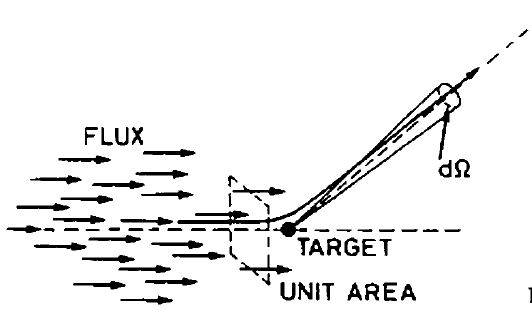
\includegraphics[width=\columnwidth]{crossection.png}
     \caption{CDiagram showing the cross section-\cite{leo1988techniques}}
     \label{CSdiag}
\end{figure}

So, the total cross section is given by:

\begin{equation}
    \sigma(E)=\int d \Omega \frac{d \sigma}{d \Omega}
\end{equation}


Assuming that the target centers are uniformly distributed and 
the slab is not too thick so that the likelihood of one center sitting 
in front of another is low, the number of centers per unit perpendicular 
area which will be seen by the beam is then $N\delta x$ where N is the 
density of centers and $\delta x$ is the thickness of the material along 
the direction of the beam. If the beam is broader than the target and A is 
the total perpendicular area of the target, the number of incident particles 
which are eligible for an interaction is then FA. The average number scattered 
into $d\Omega$ per unit time is then:

\begin{equation}
    N_s(\Omega) = FAN\delta x \frac{d\sigma}{d\Omega}
\end{equation}

and,

\begin{equation}
    N_{tot} = FAN \delta x \sigma
\end{equation}

And the probability of interaction in $\delta x$ is $N\sigma \delta x$-\cite{leo1988techniques}

\subsection{Interaction Probability}

Here we will calculate what id probability that a particle does not involve
in an interaction for a distance of x, this probability is known as the 
survival probability $P(x)$. Let the probability of having an interaction between 
$x$ and $dx$ be $wdx$. Then we have the probability of not having an interaction
between $x$ and $x+dx$ as:

\begin{equation}
    P(x+dx) = P(x)(1-wdx)
\end{equation}

On solving, we get the P(x) as :
\begin{equation}
    P(x) = C\exp{-wx}
\end{equation}
C turns out to be 1 while substituting the usual probability properties.


Now as we have the interaction probability, we will calculate the mean free
path, which is defined as:
\begin{equation}
    \lambda = \frac{\int x P(x)dx}{\int P(x)dx} = \frac{1}{w}
\end{equation}

but the interaction probability depends on the $\delta x$ intuitively, after 
approximating to the linear order terms we get:
\begin{equation}
    \lambda = \frac{1}{N\sigma}
\end{equation}


So the survival probability becomes:

\begin{equation}
    P(x) = \exp{(\frac{-x}{\sigma})}=\exp{(-N\sigma x)}
\end{equation}


\subsection{Energy Loss of the penetrating particle by Atomic Collisions}

Inelastic collisions with atomic electrons and the elastic scattering from the nuclei
are the two main reasons for the energy loss and change in direction of the particle.

Of course, the inelastic collisions are statistical in nature and have a 
certain quantum mechanical probability of happening. The fluctuations in 
the total energy loss are, however, small due to their abundance per 
macroscopic path length, so one can effectively work with the average 
energy loss per unit path length. Bohr first calculated this quantity 
often referred to as the stopping power or simply dE/dx—using classical 
reasoning. Later, Bethe, Bloch, and others did so using quantum mechanics.


\subsubsection{Bohr's Calculation}

Consider a heavy particle traveling through a material medium with a 
charge ze, mass M, and velocity v. Assume that an atomic electron is 
present at a distance and from the particle trajectory as shown in 
Figure-\ref{bohrsct1} 
In order to capture the electric field acting 
on the electron at its initial position, we assume that the electron 
is free, initially at rest, and that it only moves very slightly during 
the interaction with the heavy particle. Furthermore, because of its much 
greater mass (M>m), we assume that the incident particle will have 
essentially maintained its original course after the collision. 
This is one justification for separating heavy particles from electrons!




\begin{figure}[H]
    \centering	
     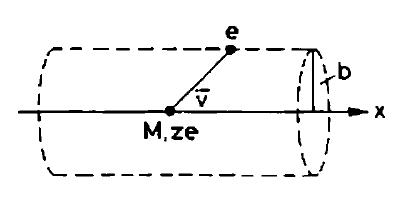
\includegraphics[width=\columnwidth]{bohrsct.png}
     \caption{Diagram For Bohr Calculation of Scattering-\cite{leo1988techniques}}
     \label{bohrsct1}
\end{figure}


Now, we will calculate the energy gained by the electron by finding the momentum impulse
it receives by colliding with the heavy particle.so:
\begin{equation}
    I = \int F dt = e\int E_{\perp} dt =e\int E_{\perp} \frac{dx}{v}
\end{equation}



By applying the gauss law, we get,

\begin{equation}
    \int E_{\perp} 2\pi bdx = 4\pi ze 
\end{equation}

So that we have:

\begin{equation}
    I = \frac{2ze^2}{bv}
\end{equation}

The energy gained by the electron is then:
\begin{equation}
    \label{eq1}
    \Delta E(b) = \frac{I^2}{2m_e} \frac{2z^2e^4}{mev^2b^2}
\end{equation}

Now, let the density of particles be $N_e$, then the energy lost to all the electrons
in the range b to b+db is given by:
\begin{equation}
    -dE(b) = \Delta E(B) N_e dV = \frac{4\pi z^2e^4}{mev^2} N_e \frac{db}{b} dx
\end{equation}

On solving with volume element $dV = 2\pi b db dx$ we get:

\begin{equation}
    -\frac{db}{dx} = \frac{4\pi z^2 e^4}{m_e v^2}N_e \ln{(\frac{b_{max}}{b_{min}})}
    \label{bmaxbmin}
\end{equation}

Ideally the limit should be 0 to infinity, but due to our assumption that
the collision at large b wont take place over a short period of time, there is an upper bound
$b_{max}$ and also at b=0, the integral diverges so there is also a $b_{min}$.

To calculate the $b_{min}$, the maximum kinetic energy is transferred when there is
a head on collision and the maximum energy it can gain is $\frac{1}{2}m_e (2v)^2$,
taking relativity we get this energy as $2\gamma^2 m_e v^2 $
substituting this to Equation-\ref{eq1}, we get,
\begin{equation}
    b_{min} = \frac{ze^2}{\gamma m_e v^2}
\end{equation}



Now for the calculation of $b_{max}$, We should look at the electrons. These electrons are not Free but bound to an atoms with some
orbital frequency $\nu$. For the electron to absorb some energy, the perturbation caused by the incident particle 
should be for a short time as compared to the angular frequency (1/$\nu$). Otherwise the perturbation 
will be adiabatic and there will be no transfer od energy. For Collisions, the interaction time is $t=b/v$. Considering the
relativistic effects, t becomes $t/\gamma$. so we can write:
\begin{equation}
    \frac{b}{\gamma v} \le \tau = \frac{1}{\bar{\nu}}
\end{equation}
where $\bar{nu}$ is the mean frequency averaged over all the states. The the upper limit of b becomes:
\begin{equation}
    b_{max} = \frac{\gamma v}{\bar{\nu}}
\end{equation}

Now substituting this into the Equation-\ref{bmaxbmin}, we get the classical bohr formula for the Energy Loss as:-\cite{leo1988techniques}

\begin{equation}
    -\frac{db}{dx} = \frac{4\pi z^2 e^4}{m_e v^2}N_e \ln{(\frac{\gamma^2 m_e v^3}{z e^2 \bar{\nu}})}
    \label{classicalbohr}
\end{equation}



\subsubsection{The Bethe-Bloch Formula}


The more realistic Quantum mechanical formulation of the Energy loss is carried out by
Bethe and Bloch in which the Energy is parametrized in terms of momentum rather than
the impact parameter. The formula thus obtained is:

\begin{equation}
    -\frac{db}{dx} = 2 \pi N_a r_e^2 C^2 \rho \frac{z^2 Z}{A \beta^2} (\ln{(\frac{2 m_e \gamma^2 v^2 W_{max}}{I^2})}-2\beta^2)
\end{equation}
Where $r_e$ is the electron radius, $N_a$ is the Avogadro Number, $\rho$ is the density of the material,
$m_e$ is the electron mass, I is the mean excitation potential, Z and A are the atomic
number and atomic mass of the absorbing material, z is the charge of the incident particle in units of e,
$W_{max}$ is the maximum energy transfer in a single collision, $\beta$ and $\gamma$ have the usual
definition in terms of velocity of the incident particle.

The maximum Energy Transfer id given by the formula:
\begin{equation}
    W_{max} = \frac{2m_e c^2 \eta^2}{1+2s\sqrt{1+\eta^2}+s^2}
\end{equation}
where $s=m_e/M$, where M is the mass of the incident particle and $\eta=\beta\gamma$.

Normally, two corrections are also added to the bethe bloch formula which is then given by:



\begin{eqnarray}
        -\frac{db}{dx} = 2 \pi N_a r_e^2 C^2 \rho \times\frac{z^2 Z}{A \beta^2} \times (\ln{(\frac{2 m_e \gamma^2 v^2 W_{max}}{I^2})} \\ -2\beta^2 - \delta - 2\frac{C}{Z})
\end{eqnarray} 


Where C is the Shell Correction and $\delta$ is the density Correction.


\section{Simulation Using Geant4}


Geant4-\cite{agostinelli2003geant4}, short for "Geometry and Tracking 4," is a powerful and 
widely-used toolkit for simulating the interactions of particles with matter. 
Developed by the CERN collaboration and used extensively in high-energy physics, 
nuclear physics, and other scientific fields, Geant4 is renowned for its accuracy 
and versatility. The toolkit provides a comprehensive set of tools and 
libraries that allow researchers to design complex geometries, define 
various particle sources, and study the interactions of particles with matter 
in intricate detail. Its modular and extensible architecture makes it adaptable 
to a wide range of simulation tasks, from studying the behavior of elementary 
particles in particle accelerators to modeling radiation therapy treatments in 
medical physics.


\subsection{The Detector Geometry}

The Detector Geometry is defined almost same as that is present in the laboratory to detect the muons. The Detector
construction is implemented using G4box, G4Tubs and G4Polyhedra. The logical volumes are crated using the G4LogicalVolume
and it is placed in appropriate positions just like what we have in the lab.

The detector that we are using in the lab is a Cosmic flux Photon Multiplicity Detector (CofPMD) in which we will be detecting
the Muons using the $Ar+CO_2$ (9:1) mixture present in the detector. So We will be setting the Sensitive detector as the Logical volume
of the Gas mixture. Using this Sensitive Detector, we will Measure the position of incidence and the Total  Energy deposition
from the Sensitive Detector.

\subsubsection{The Honeycomb shaped Detector}

Our main part of the detector is a honeycomb shaped detector made up of Copper in which at the Centre of each
hexagon there is a thin gold wire and this acts as the Anode in the real case and the Cu part acts as the Cathode. This whole
honeycomb is filled with a Mixture of Argon and Carbon Dioxide in the ratio 9:1. The Inner Radius of the Hexagon is $2.5mm$
and its depth is $5mm$. The radius of the Gold wire present at the centre is 10 microns. The construction of the honeycomb
and the gold wire is done using G4Polyhedra and G4Tubs respectively. The Constructed Hexagonal Honeycomb Structure is 
shown in the Figure-\ref{honeycomb}.

\begin{figure}[H]
    \centering	
     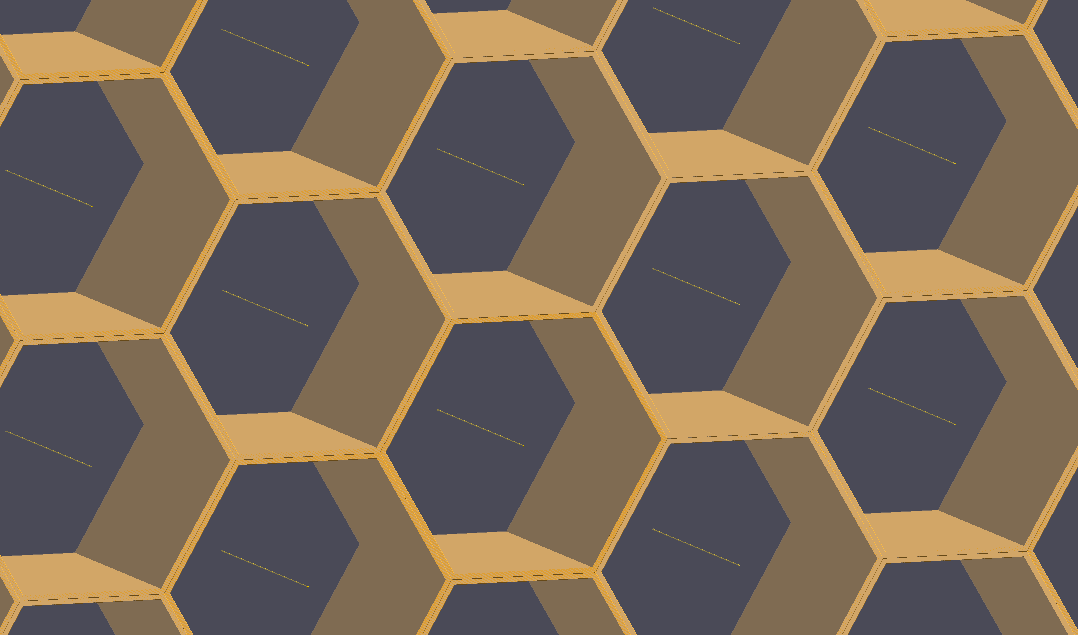
\includegraphics[width=\columnwidth]{honeycomb.png}
     \caption{Honeycomb structure created from GEANT4}
     \label{honeycomb}
\end{figure}

\begin{figure}[H]
    \centering	
     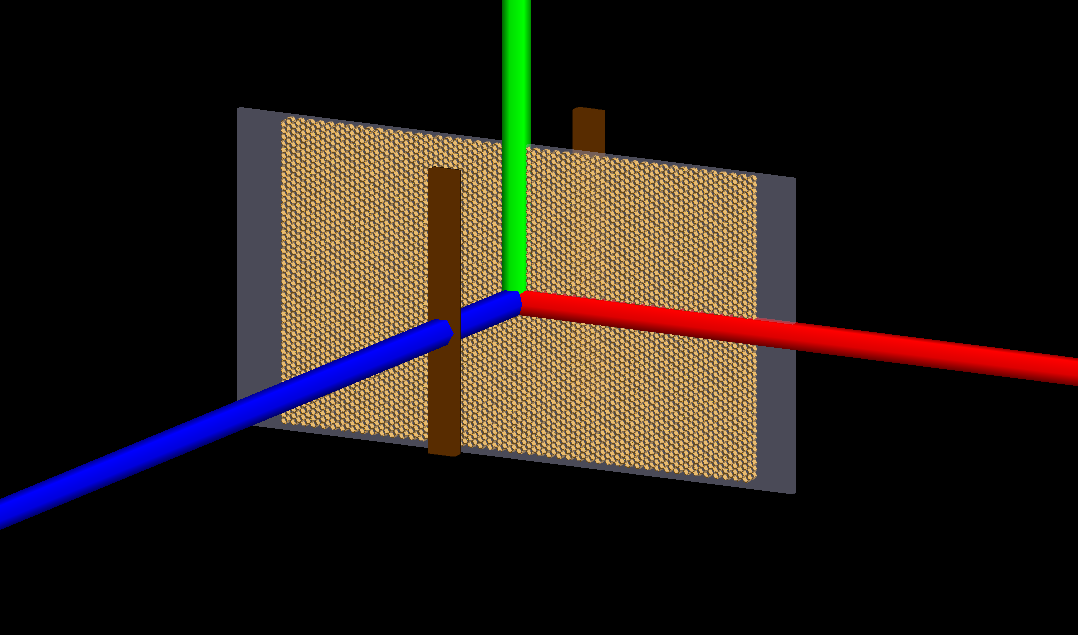
\includegraphics[width=\columnwidth]{honeycomb1.png}
     \caption{Honeycomb structure and Scintillation detectors created from GEANT4 (The RED BLUE and GREEN Lines are x,z and y axes)}
     \label{honeycomb1}
\end{figure}
The detector also contains Two scintillation detectors (of Thickness 1 cm and length of 11cm)  which are placed one above and one below at equal distances of 11cm
from the honeycomb detector. This is shown in the Figure-\ref{honeycomb1}







\subsubsection{The Complete Setup}

The complete Setup of the Experiment is implemented using the Detector
construction in GEANT4. The Complete construction is Shown in the 
Figure-\ref{combsetup}. The Grey parts of the simulations are made up
of Aluminum and the green parts are made up of plastic. Also the Electronics and
the PMDs are constructed whose material is FR4.

\begin{figure}[H]
    \centering	
     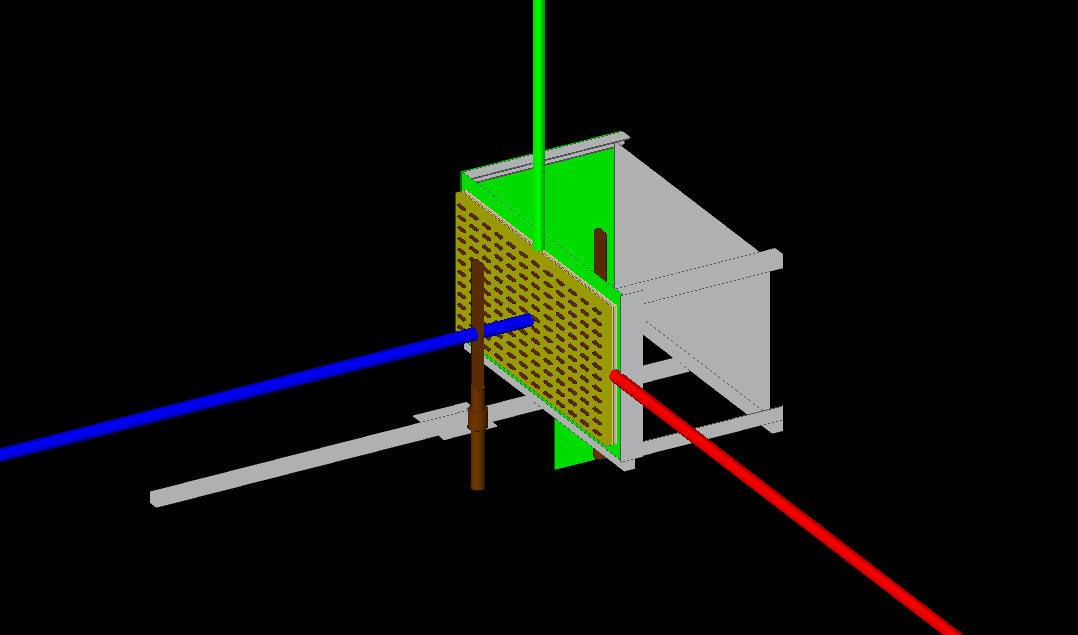
\includegraphics[width=\columnwidth]{combsetup.png}
     \caption{The complete Experimental Setup Simulation}
     \label{combsetup}
\end{figure}





\subsection{Generation of Particles}

The particle generation and its projection is done using the
usual fParticleGun with the G4VUserPrimaryGeneratorAction in Geant4.
Using this one can generate as many particles as we want in a single run.
for our case we will be generating muons only for the single particle case and
and for the Actual simulation of the Cosmic Shower, we will be using the
EcoMug for the data for different types of particles.




\subsection{Collection of Energy Deposition Data}
The energy Deposit form the Gas Mixture is calculated by the 
sensitive detector which was assigned for the Argon Gas mixture.
Geant4 Calculates the Energy Deposits and then it writes the values
for each run (each run consist of shooting of a single muon perpendicular to the 
Gas detector) into a text file. Which is then read by the Python and ROOT for further analysis.
The implementation  of the Detection and its calculation is 
done using G4VSensitiveDetector and G4Track.





\section{Single Muon Interaction}

In this case, we will be using the fParticleGun to Generate $\mu^-$-Particles 
and will project them to the Detector through the scintillation detector 
parallel to the Z-Axis. We will be defining the momentum in terms of Energy (MeV and GeV) and all of this
with Construction of the detectors as mentioned above. 


\subsection{Obtained Energy Deposit data}

As mentioned earlier, the $\mu^-$-particles are fired at different
energies. Then its Most probable Energy Deposit Values are taken 
and plot against the incident energy and the graph is Checked by the
bethe-bloch formula.


\subsubsection{Single Energy Muon}

At first, we fired one particle at 4GeV perpendicular
to the detector through the scintillator in one run (100000 Runs were made). The plot of the range of
Energy Deposit is Shown in the Figure-\ref{ED4GeV} where we can see
that the distribution is landau. The function is Fitted by the
Landau function and MPV of the Energy Deposit is obtained as 515.87eV and the standard deviation
is 165.912eV. The corresponding image of the accumulated paths of the muons
as shown in the Figure-\ref{ED4GeVaccu}
\begin{figure}[H]
    \centering	
     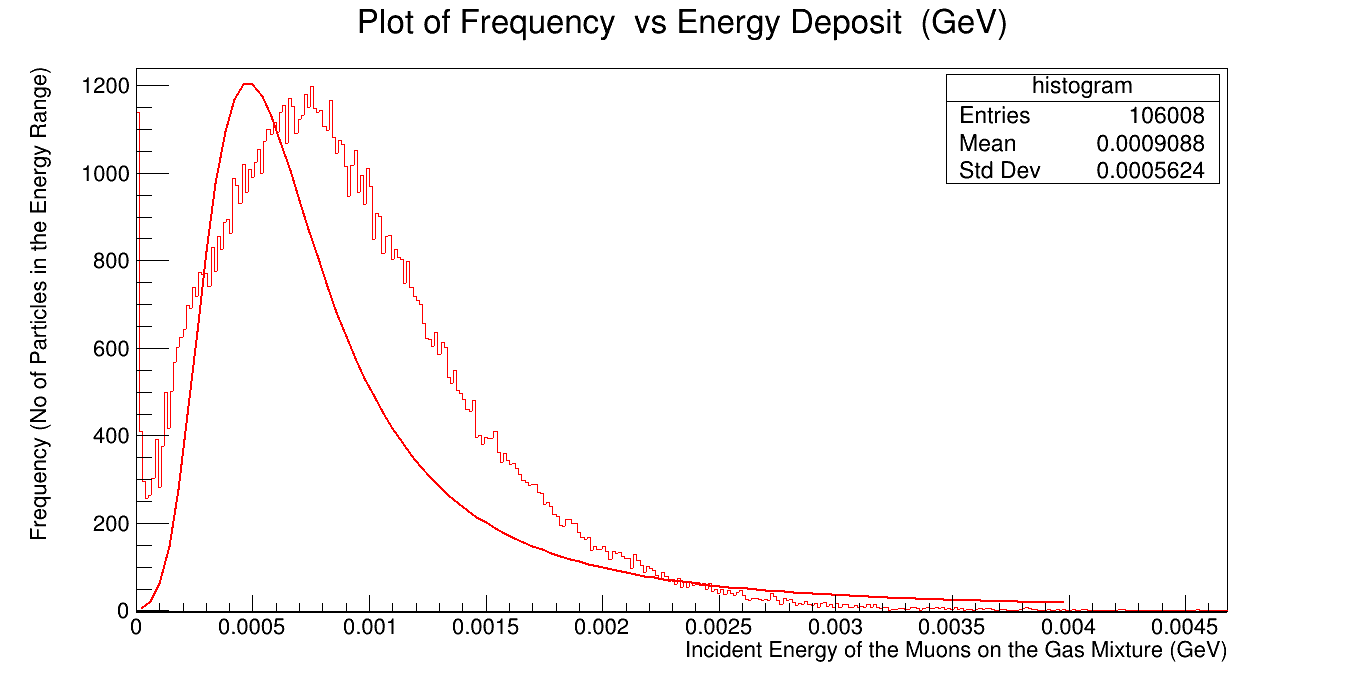
\includegraphics[width=\columnwidth]{ED4GeV.png}
     \caption{Statistics of Energy Deposit by 4GeV Muon Minus-\cite{ROOT}}
     \label{ED4GeV}
\end{figure}

\begin{figure}[H]
    \centering	
     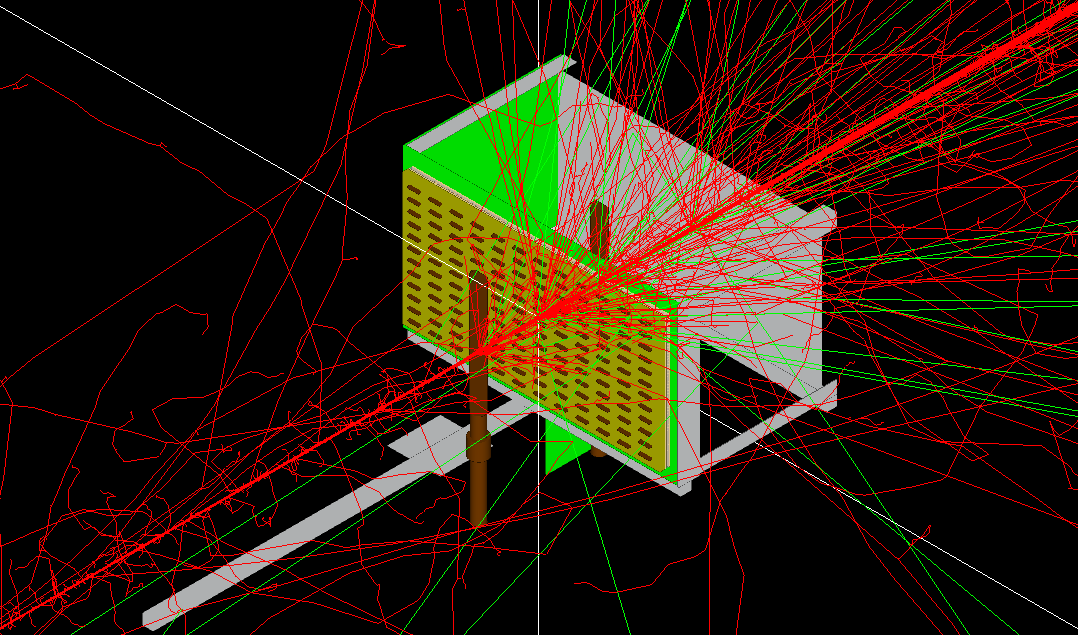
\includegraphics[width=\columnwidth]{ED4GeVaccu.png}
     \caption{Accumulated paths of the muons for 500 Runs-\cite{agostinelli2003geant4}}
     \label{ED4GeVaccu}
\end{figure}


\subsubsection{Muons With Different Energies}

Now, we will be calculating the Most Probable Value (MPV) of the
Energy Deposit for different values of the incident energy. We will Start 
from low energy (80MeV) and will end at calculating MPV of each Energy deposition
till we reach 100GeV particles. For Each energy we will be firing 100000 $\mu^-$-particles
one by one for each run. The energy Deposit is Calculated by the Sensitive Detector 
(Argon+$CO_2$ Mixture)





















\end{multicols}
\bibliographystyle{plain}
\bibliography{bib.bib}


\end{document}